\documentclass[11pt]{article}

\usepackage[english]{babel}
\usepackage[T1]{fontenc}
\usepackage[utf8x]{inputenc}

\usepackage{appendix}
\usepackage{amsmath}
\usepackage{cprotect}
\usepackage{listings}
\usepackage{float}
\usepackage[margin=2cm]{geometry}
\usepackage{graphicx}
\usepackage{underscore}
\usepackage{subcaption}

\graphicspath{ {assets/exer001/} }

\lstset{
    tabsize=3,
    breakatwhitespace=true,
    breaklines=true,
    frame=simple
}

\title{Exercise 1 - FPGA Simulated Annealing with VPR}
\author{Matthew Walker - 999540475 - walker82}
\date{\today}

% Placement
%   DONETODO score vs. temp (for each circuit)
%   DONETODO mean and stddev for at least 5 seeds
%   DONETODO add bump-up capability, repeat previous
%   DONETODO 5 temps X 5+ seeds, be sure to impact solution

% Routing
%   DONETODO run routing with W set, report post-routing crit. path delay
%   vary params to improve fmax
%   change pin-within-net and net ordering, report fmax

\begin{document}

\maketitle

\section{Simulated Annealing Placement}
\subsection{Baseline HPWL Placer}
\subsubsection{Cost vs Time/Temperature Plots}
\begin{figure}[ht]
\subcaptionbox{bigkey}{
	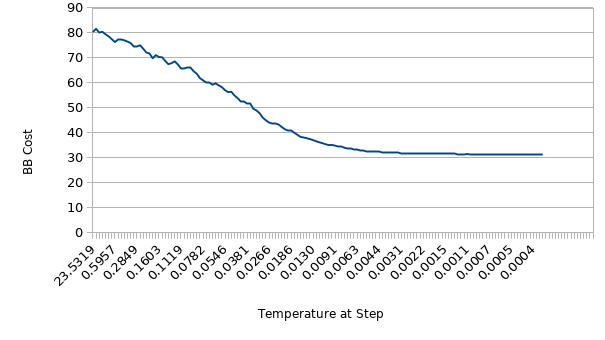
\includegraphics[width=0.5\linewidth]{bigkey-cost-at-step}}
\subcaptionbox{mkSMAdapter4B}{
	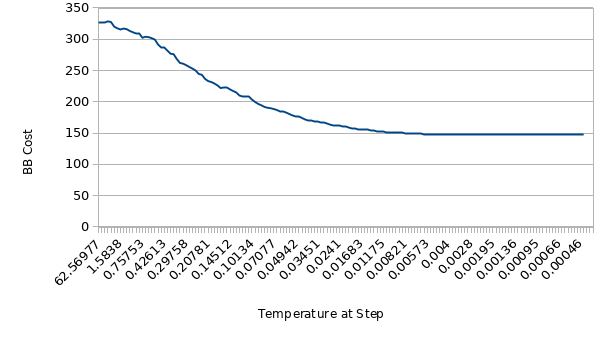
\includegraphics[width=0.5\linewidth]{mk-cost-at-step}}
\subcaptionbox{or1200}{
	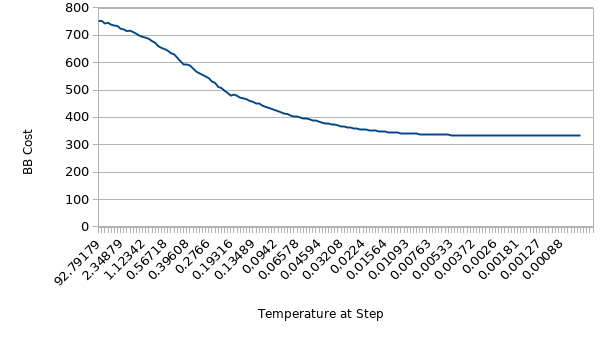
\includegraphics[width=0.5\linewidth]{or1200-cost-at-step}}
\subcaptionbox{pair}{
	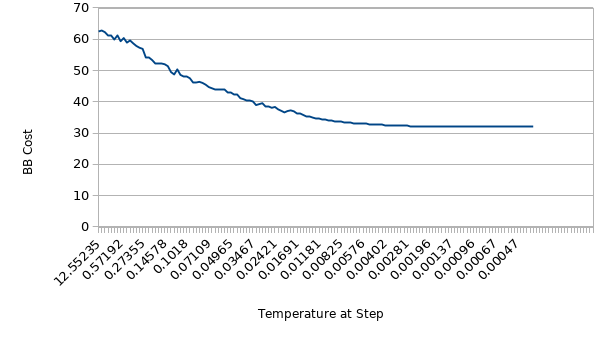
\includegraphics[width=0.5\linewidth]{pair-cost-at-step}}
\caption{HPWL cost over the course of placement (x \(\propto\) step number), with temperature labels.}
\label{fig:baseline-hpwl}
\end{figure}

\subsubsection{Seed Effects}

\begin{table} \centering
\begin{tabular}{l | *4r}
\hline\hline
circuit\textbackslash statistic & total blocks & total nets & total inputs & total outputs \\
\hline
bigkey & 1333 & 1136 & 229 & 197 \\
mkSMAdapter4B & 3513 & 3308 & 195 & 205 \\
or1200 & 4589 & 4258 & 385 & 394 \\
pair   & 791  &  654 & 173 & 137 \\
\hline\hline
\end{tabular}
\caption{Circuit statistics, after removing unused inputs.}
\label{tab:circuit-stats}
\end{table}

\begin{table}
\centering
\begin{tabular}{l | *{15}r}
\hline\hline
circuit\textbackslash init temp & 0.015 & 0.03 & 0.05 & 0.1 & 0.5 & 1 & 5 & 20 & 50 & default (100)\\
\hline
bigkey & 0.98 & 1.43 & 1.39 & 0.56 & 0.54 & 0.91 & 0.75 & 1.01 & 1.09 & 1.03 \\
mkSMAdapter4B & 4.73 & 3.96 & 5.25 & 3.62 & 1.93 & 2.65 & 1.97 & 2.21 & 1.59 & 1.81 \\
or1200 & 7.88 & 8.80 & 5.83 & 9.42 & 5.45 & 4.54 & 5.57 & 3.75 & 4.96 & 2.71 \\
pair & 1.22 & 0.76 & 0.76 & 0.45 & 0.62 & 0.62 & 0.39 & 0.52 & 0.37 & 0.36 \\
\hline\hline
\end{tabular}
\caption{Standard deviation of the final cost of 10 seeds of each circuit with various initial temperature settings. Default temperature adjustment schedule. }
\label{tab:stddev-by-temp}
\end{table}

\begin{table}
\centering
\begin{tabular}{l | *{15}r}
\hline\hline
circuit\textbackslash init temp & 0.015 & 0.03 & 0.05 & 0.1 & 0.5 & 1 & 5 & 20 & 50 & default (100)\\
\hline
bigkey & 2.3 & 3.6 & 3.8 & 1.6 & 1.4 & 2.4 & 2.0 & 2.7 & 2.9 & 3.3 \\
mkSMAdapter4B & 2.4 & 2.2 & 3.1 & 2.2 & 1.2 & 1.7 & 1.2 & 1.4 & 1.0 & 1.2 \\
or1200 & 1.8 & 2.2 & 1.5 & 2.5 & 1.5 & 1.3 & 1.6 & 1.0 & 1.4 & 0.8 \\
pair & 3.2 & 2.1 & 2.2 & 1.3 & 1.8 & 1.8 & 1.2 & 1.5 & 1.1 & 1.1 \\
\hline\hline
\end{tabular}
\caption{Standard deviation of the final cost of 10 seeds of each circuit with various initial temperature settings, as a percentage of the mean. Default temperature adjustment schedule. }
\label{tab:stddev-by-temp-as-percent}
\end{table}

\begin{table}
\centering
\begin{tabular}{l | *{15}r}
\hline\hline
circuit\textbackslash init temp & 0.015 & 0.03 & 0.05 & 0.1 & 0.5 & 1 & 5 & 20 & 50 & default (100)\\
\hline
bigkey & 42.7 & 39.2 & 37.0 & 36.2 & 37.8 & 37.9 & 38.1 & 37.5 & 37.1 & 31.4 \\
mkSMAdapter4B & 194.8 & 176.7 & 169.6 & 164.9 & 158.9 & 159.8 & 158.7 & 159.0 & 160.6 & 148.8 \\
or1200 & 438.7 & 401.4 & 383.9 & 375.2 & 359.4 & 359.8 & 359.4 & 359.0 & 358.5 & 333.7 \\
pair & 38.4 & 35.9 & 34.5 & 34.1 & 34.1 & 33.9 & 33.7 & 33.7 & 33.7 & 31.5 \\
\hline\hline
\end{tabular}
\caption{Mean final cost of 10 seeds of each circuit with various initial temperature settings. Default temperature adjustment schedule. }
\label{tab:mean-by-temp}
\end{table}

The circuits are similarly affected by noise when the standard deviation across seeds is normalized as a fraction of the mean (table \ref{tab:stddev-by-temp-as-percent}). However, when considered in absolute terms, the largest circuit, \emph{or1200} (see table \ref{tab:circuit-stats}), has the largest variation. Also, \emph{or1200}'s final cost is considerably higher than the only-slightly-smaller circuit \emph{mkSMAdapter4B}, suggesting that it has a significantly more difficult placement problem. Finally, there seems to be some dependency on circuit, as \emph{bigkey} has a somewhat larger variance, but middling statistics offering no explanation.

\subsection{Modifying the Temperature Change Schedule}

\begin{table}
\centering
\begin{tabular}{l | *{15}r}
\hline\hline
circuit\textbackslash bump frac. & 0.01 & 0.05 & 0.1 & 0.5 \\
\hline
bigkey & 1.54 & 0.68 & 1.03 & 0.96 \\
mkSMAdapter4B & 1.36 & 2.81 & 1.81 & 2.52 \\
or1200 & 2.88 & 2.67 & 2.71 & 1.30 \\
pair & 0.50 & 0.46 & 0.36 & 0.37 \\
\hline\hline
\end{tabular}
\caption{Standard deviation of the final cost of 10 seeds of each circuit with various degrees of bumping. }
\label{tab:stddev-by-temp-bump}
\end{table}

\begin{table}
\centering
\begin{tabular}{l | *{15}r}
\hline\hline
circuit\textbackslash bump frac. & 0.01 & 0.05 & 0.1 & 0.5 \\
\hline
bigkey & 4.8 & 2.2 & 3.3 & 3.0 \\
mkSMAdapter4B & 0.9 & 1.9 & 1.2 & 1.7 \\
or1200 & 0.9 & 0.8 & 0.8 & 0.4 \\
pair & 1.6 & 1.5 & 1.1 & 1.2 \\
\hline\hline
\end{tabular}
\caption{Standard deviation of the final cost of 10 seeds of each circuit with various degrees of bumping, as a percentage of the mean. }
\label{tab:stddev-by-temp-as-percent-bump}
\end{table}

\begin{table}[h]
\centering
\begin{tabular}{l | *{15}r}
\hline\hline
circuit\textbackslash bump frac. & 0.01 & 0.05 & 0.1 & 0.5 \\
\hline
bigkey & 32.2 & 31.4 & 31.4 & 31.8 \\
mkSMAdapter4B & 148.4 & 148.3 & 148.8 & 149.7 \\
or1200 & 333.9 & 332.9 & 333.7 & 332.3 \\
pair & 31.5 & 31.3 & 31.5 & 31.4 \\
\hline\hline
\end{tabular}
\caption{Mean final cost of 10 seeds of each circuit with various degrees of bumping. }
\label{tab:mean-by-temp-bump}
\end{table}

Examining the values in table \ref{tab:mean-by-temp-bump}, and comparing to the final column of table \ref{tab:mean-by-temp}, there is a significant difference when temperature bumping is added. The bumping scheme used was to wait until the placement would exit normally, then set the temperature instead to a (fractional) multiple of the initial temperature ("bump factor"). This would only activate once, and the second time the temperature reached the exit condition, placement will stop.

\section{Timing-Driven Pathfinder Routing}
\subsection{Parameter Exploration}
The initial present cost, present cost multiplier, A* factor, and accumulation factor were swept and combined, as presented in table \ref{tab:param-data}. The change with the most effect was a decrease of the present cost multplier from 1.3 to 1.05, and in particular when combined with a decrease in the initial present cost from 0.5 to 0.4. The decrease was largest when this was combined with a slight decrease in the A* factor from 1.2 to 1.1. The generally lower and slower growing present congestion costs should reduce pressure for the circuit to converge, and allow the circuit to settle slower and on better solutions. The decrease in the A* factor contributed by making sure that better paths were explored. These changes cause the circuits to take longer to route (in particular \emph{or1200}), and the maximum number of routing iterations had to be increased, which should be expected.

\begin{table}[h]\centering
\begin{tabular}{l | *{9}r}
\hline\hline
circuit & \scriptsize  default & \scriptsize  $P_{f_0} = 0.4$ & \scriptsize  $P_{f_0} = 0.25$  & \scriptsize   $P_m = 1.05$ & \scriptsize   $P_m = 1.1$ & \scriptsize   $P_m = 1.2$ & \scriptsize  $C_{astar} = 1.15$ \\
\hline
bigkey & 2.43 & 2.43 & 2.43 & 2.43 & 2.43 & 2.49 & 2.40 \\
mkSMAdapter4B & 5.56 & 5.83 & 5.72 & 5.42 & 5.44 & 5.44 & 5.65 \\
or1200 & 13.33 & 13.31 & 13.38 & 12.81 & 12.88 & 13.21 & 13.09 \\
pair & 3.11 & 3.15 & 3.15 & 3.00 & 3.06 & 3.12 & 3.14 \\
\hline
geomean & 4.87 & 4.94 & 4.92 & 4.74 & 4.78 & 4.86 & 4.86 \\
\end{tabular}
\begin{tabular}{l *{9}r}
\hline\hline
\scriptsize  $C_{astar} = 1.1$ & \scriptsize  $C_{astar} = 1.05$ & \scriptsize  $A = 0.95$ & \scriptsize  $A = 0.9$ & \scriptsize  $A = 0.85$ & \scriptsize  $P_{f_0} = 0.4$   $P_m = 1.1$ & \scriptsize  $P_{f_0} = 0.4$   $P_m = 1.2$ \\
\hline
2.45 & 2.45 & 2.50 & 2.43 & 2.43 & 2.43 & 2.43 \\
5.52 & 5.59 & 5.76 & 5.66 & 5.76 & 5.44 & 5.57 \\
13.05 & 13.06 & 13.21 & 13.25 & 13.21 & 12.99 & 13.15 \\
3.16 & 3.09 & 3.10 & 3.18 & 3.23 & 3.08 & 3.28 \\
\hline
4.86 & 4.85 & 4.93 & 4.91 & 4.94 & 4.80 & 4.92 \\
\end{tabular}
\begin{tabular}{*{8}r}
\hline\hline
\scriptsize  $P_{f_0} = 0.25$   $P_m = 1.1$ & \scriptsize  $P_{f_0} = 0.25$   $P_m = 1.2$ & \scriptsize  $P_{f_0} = 0.4$   $P_m = 1.05$ $C_{astar} = 1.1$ & \scriptsize  $P_{f_0} = 0.4$   $P_m = 1.1$ $C_{astar} = 1.1$ $A = 0.9$ \\
\hline
2.43 & 2.43 & 2.39 & 2.44 \\
5.42 & 5.66 & 5.44 & 5.43 \\
13.18 & 13.21 & 12.81 & 12.81 \\
3.05 & 3.05 & 2.99 & 3.09 \\
\hline
4.79 & 4.85 & 4.74 & 4.79 \\
\end{tabular}
\caption{Experimental mean critical path delays across 4 seeds of each design, across various parameter settings. $P_{f_0}$ is the initial present factor cost, $P_m$ is the present factor multiplier, $C_{astar}$ is the A* factor, $A$ is the accumulation factor. If multiple parameters are specified, then all are set for that column. The maximum number of routing iterations was set to 200 for all to prevent routing failures.}
\label{tab:param-data}
\end{table}

\clearpage

\subsection{Net Ordering}

There appears to be no effect when reversing the order nets or pins are routed from the default. This is expected, as routes are negotiated, and the highly critical routes will always be the same nets, so the same nets should end up pushing out other nets and taking the routing resources they most desire.

\begin{table}[h]\centering
\begin{tabular}{l | *3r}
\hline\hline
run name &  default &  reverse pins &  reverse nets \\
\hline
bigkey & 2.43 & 2.43 & 2.43 \\
mkSMAdapter4B & 5.56 & 5.56 & 5.79 \\
or1200 & 13.33 & 13.03 & 13.34 \\
pair & 3.11 & 3.15 & 3.05 \\
\hline
geomean & 4.87 & 4.85 & 4.89 \\
\hline\hline
\end{tabular}
\caption{Mean critical path delays across 4 seeds of each design under different reversal conditions.}
\label{tab:ordering-effects}
\end{table}

\end{document}
